\documentclass[../main.tex]{subfiles}
\graphicspath{{img},{img/ink},{ink}}

\begin{document}
\begin{tcolorbox}[
    width=\textwidth,
    height=\textheight,
    title=Versuch: Die schlanke Spule,
    fonttitle=\Large,
    before title=\vspace{0.2cm}, after title=\vspace{0.2cm},
    colback=white,
    title filled=true, 
    colbacktitle=mygray,
    colframe=black,
    coltitle=black,
    ]

    \vspace{0.2cm}
    \textbf{Klassenstufe}: 11/12

    \vspace{0.5cm}

    \textbf{Fachlicher Bezug}: Magnetfeld im Inneren einer schlanken Spule

    \vspace{0.5cm}

    \textbf{Material}: Mobile-CASSY mit Hall-Sensor, Neva-Spule, Schalter, Amperemeter (min. 100 mA), stabilisierendes Netzgerät 300 V, Sicherheitskabel 
    \vspace{0.5cm}

    \begin{minipage}[c]{0.5\textwidth}
        \centering
        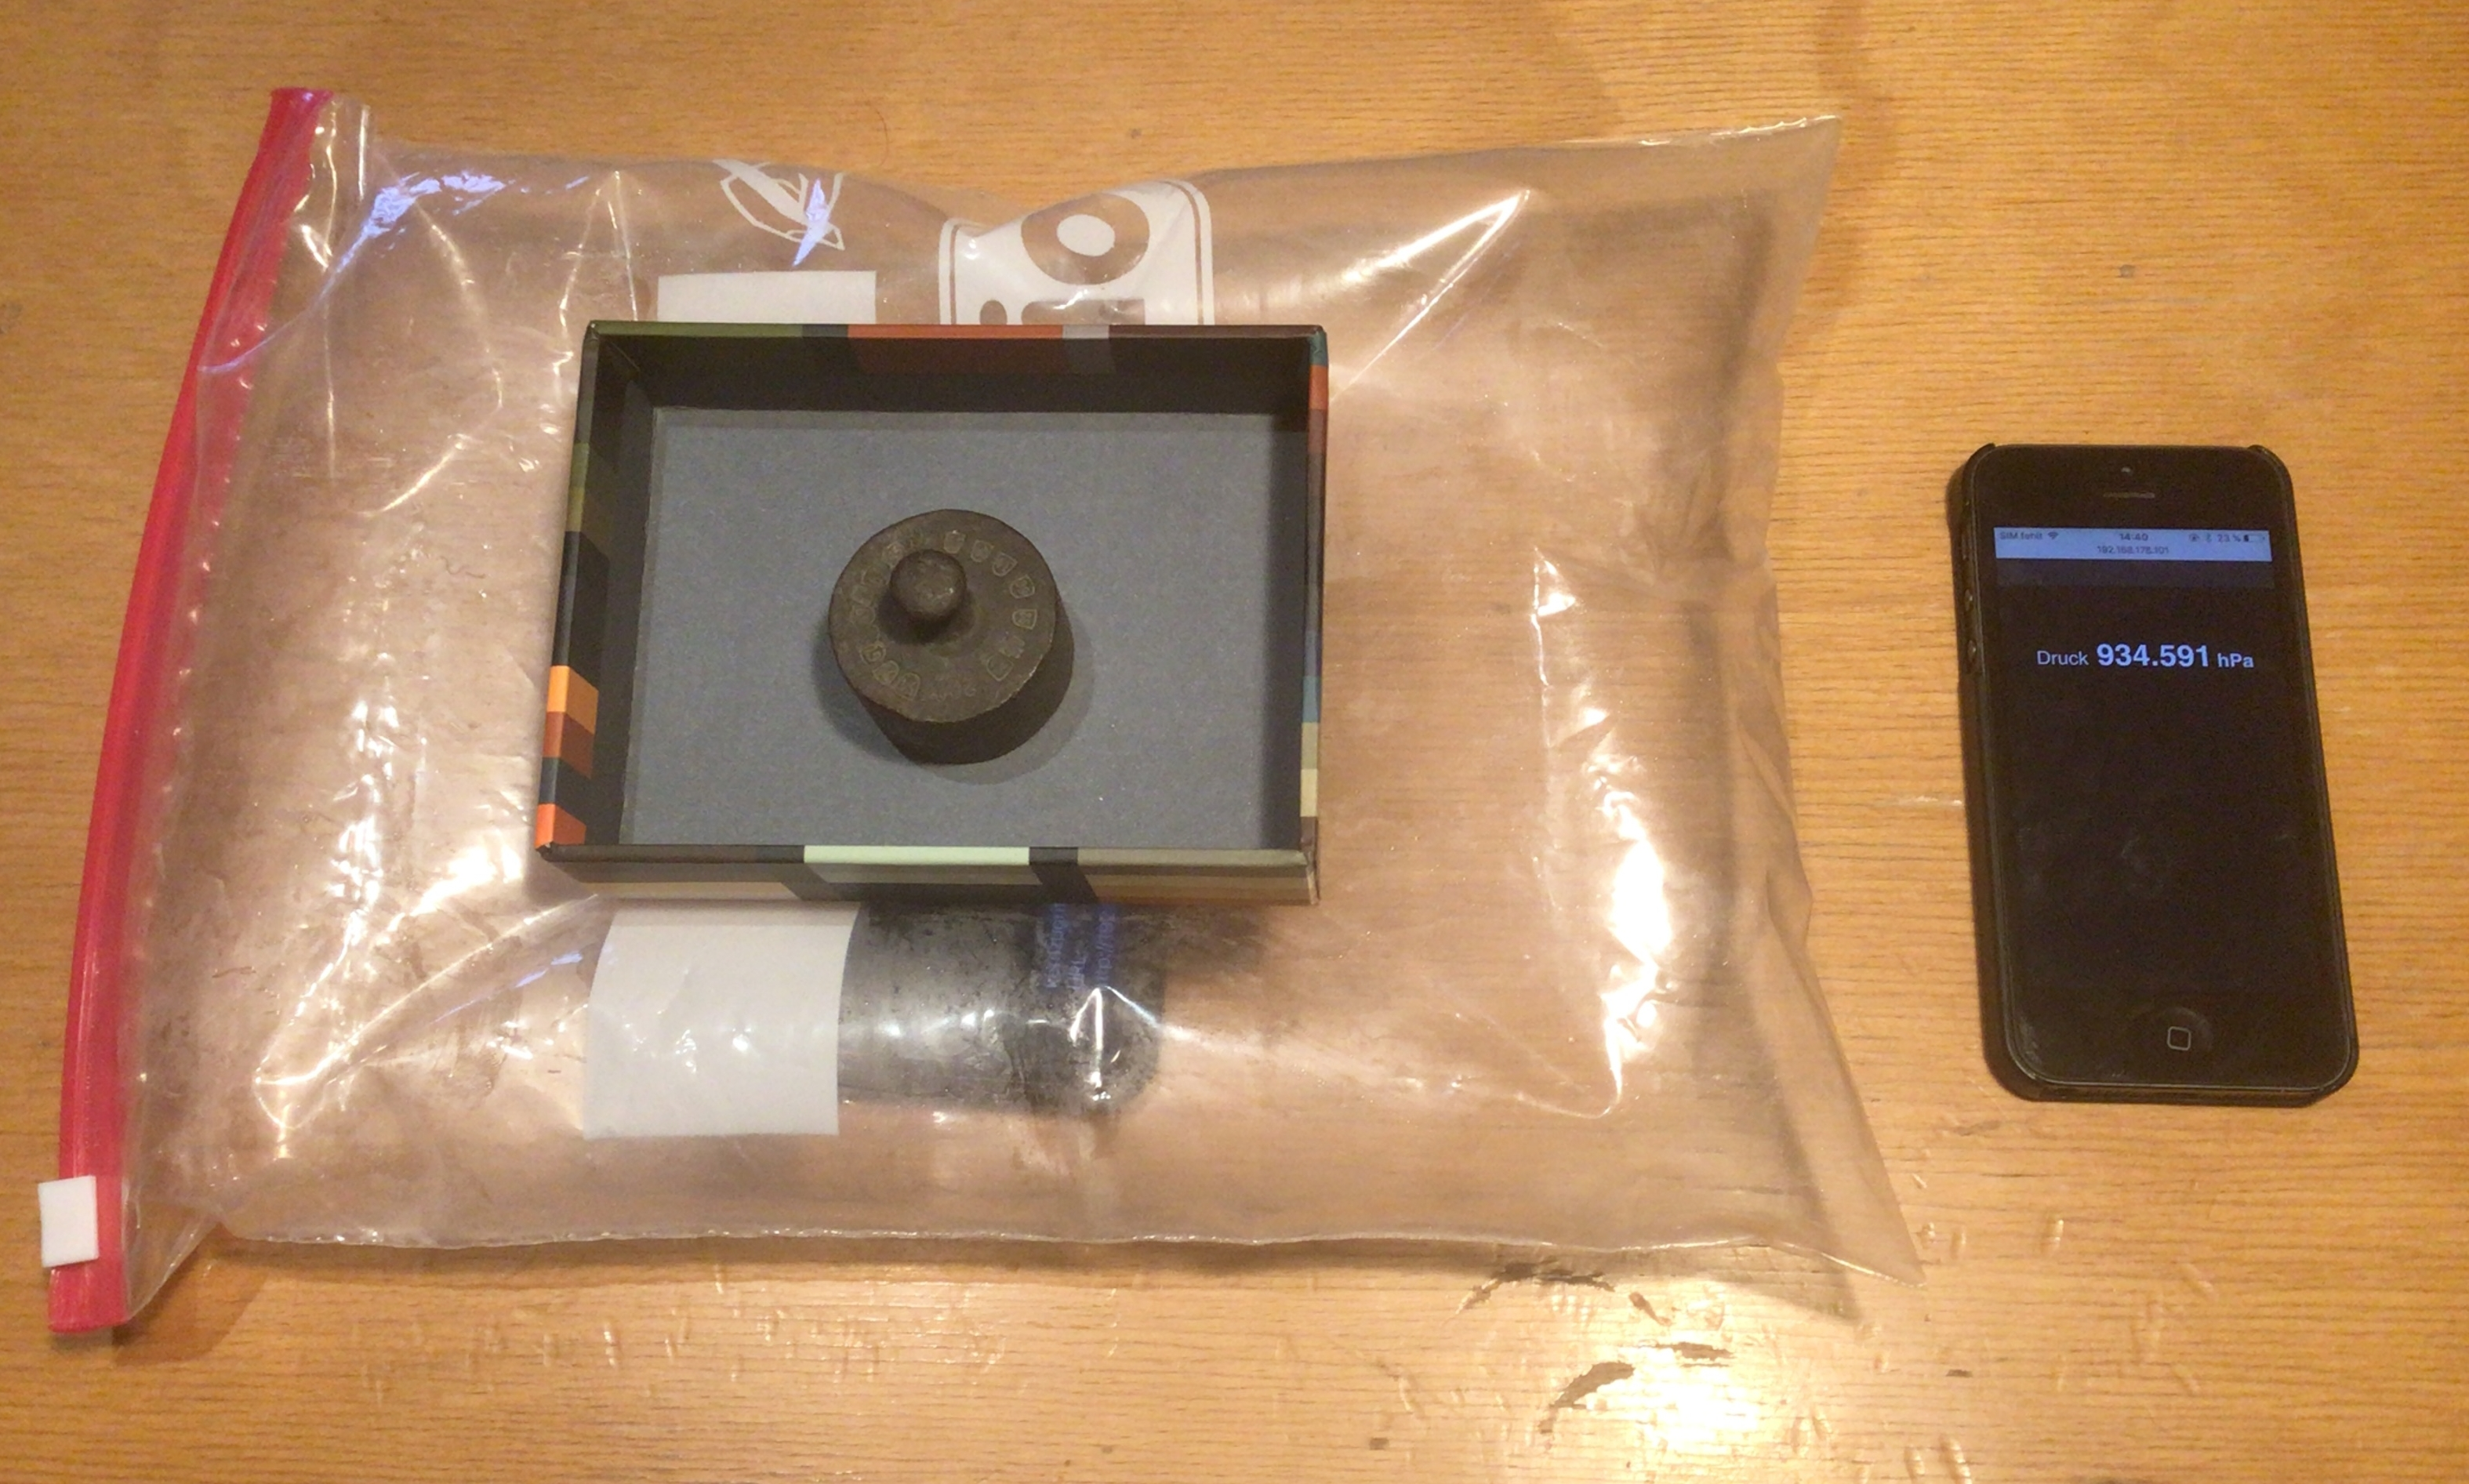
\includegraphics[width=0.9\textwidth]{img/versuchsaufbau}
    \end{minipage}
    \begin{minipage}[c]{0.5\textwidth}
        \begin{center}
            \begin{circuitikz} 
                \ctikzset{
                    bipoles/capacitor/width/.initial=.1,
                    european resistors
                }
                \draw   (0,0) node[spdt] (s) {};
                \draw (s.in) to [short] (-1,0) coordinate (l);
                \draw (s.out 1) to [inductor,l=$n_1$] ++(3,0) coordinate (c1);
                %\node at ([shift={(-1.5,0.6)}] c1)  {$n=8000$};
                \draw (s.out 2) to [inductor,l_=$n_2$] ++(3,0) coordinate (c2);
                %\node at ([shift={(-1.5,-0.5)}] c2) {$n=16000$};
                \draw (c1)--++(0,-2) coordinate (br);
                \draw (br) to [ammeter,mirror,invert] ++ (-4.6,0) coordinate (al);
                \draw (l) to [battery1] (al);
            \end{circuitikz}
        \end{center}
    \end{minipage}

    \vspace{0.5cm}
    \textbf{Aufbau}: Über einen Stativaufbau wird der Hall-Sensor des Mobile-CASSY in der Mitte einer Neva-Spule platziert. Durch einen Schalter kann zwischen den Windungen der Spule umgeschaltet werden. Ein stabilisierendes Netzgerät dient als Spannungsquelle. Zur Anzeige der Stromstärke durch die Spule wird ein Amperemeter in Reihe geschaltet.      

    \vspace{0.5cm}
    \textbf{Durchführung}: Die Abhängigkeit des Magentfelds von der Stromstärke wird bei fester Windungszahl $n_1=8000$ bestimmt. Mit Hilfe der Strombegrenzung werden $I=50$ mA eingestellt und der Messwert des Hall-Sensors am Mobile-CASSY abgelesen. Anschließend wird auf $I=100$ mA erhöht.\\
    Im nächsten Schritt wird die Abhängigkeit von der Windungszahl untersucht. Bei konstanter Stromstärke $I=100$ mA werden mit Hilfe des Schalters Werte für das Magnetfeld bei $n_1=8000$ und $n_2=16000$ Windungen aufgenommen.\\
    Um zusätzlich die magnetische Feldkonstante $\mu_0$ zu bestimmen, kann abschließend die Länge $l$ der Neva-Spule gemessen werden.

    \vspace{0.5cm}
    \textbf{Ergebnis}: Bei fester Windungszahl kann die Proportionaliät $B \sim I$ nachgewiesen werden. Bei konstanter Stromstärke beobachtet man $B \sim n$.\\
    Ausgehend von der Formel für das Magnetfeld einer Zylinderspule $B=\mu_0 \cdot \frac{I \cdot N}{l}$ kann durch Messen von $I,N$ und $l$ die magnetische Feldkonstante 
    \begin{align*}
        \mu_0 = \frac{B \cdot l}{I \cdot N}
    \end{align*}
    bestimmt werden (theoretisch: $\mu_0=4\pi$).

    \vspace{0.5cm}
    \textbf{Didaktische Bemerkungen}: Um die Proportionalität $B \sim \frac{1}{l}$ zu zeigen, kann eine zweite Neva-Spule angehängt werden. Werden zusätzlich Magnetkerne in die Spule eingeführt, lässt sich eine deutliche Verstärkung des Magnetfelds beobachten.

    \vspace{0.5cm}
    \begin{minipage}[c]{0.85\textwidth}
        \textbf{Bemerkungen}: Um die notwendige Stromstärke in der Spule zu erzeugen, wird ein Netzteil mit Hochspannung eingesetzt. Es ist auf die Verwendung von entsprechenden Sicherheitskabeln zu achten.    
    \end{minipage}
    \hspace{0.5cm}
    \begin{minipage}[c]{0.1\textwidth}
        \centering
        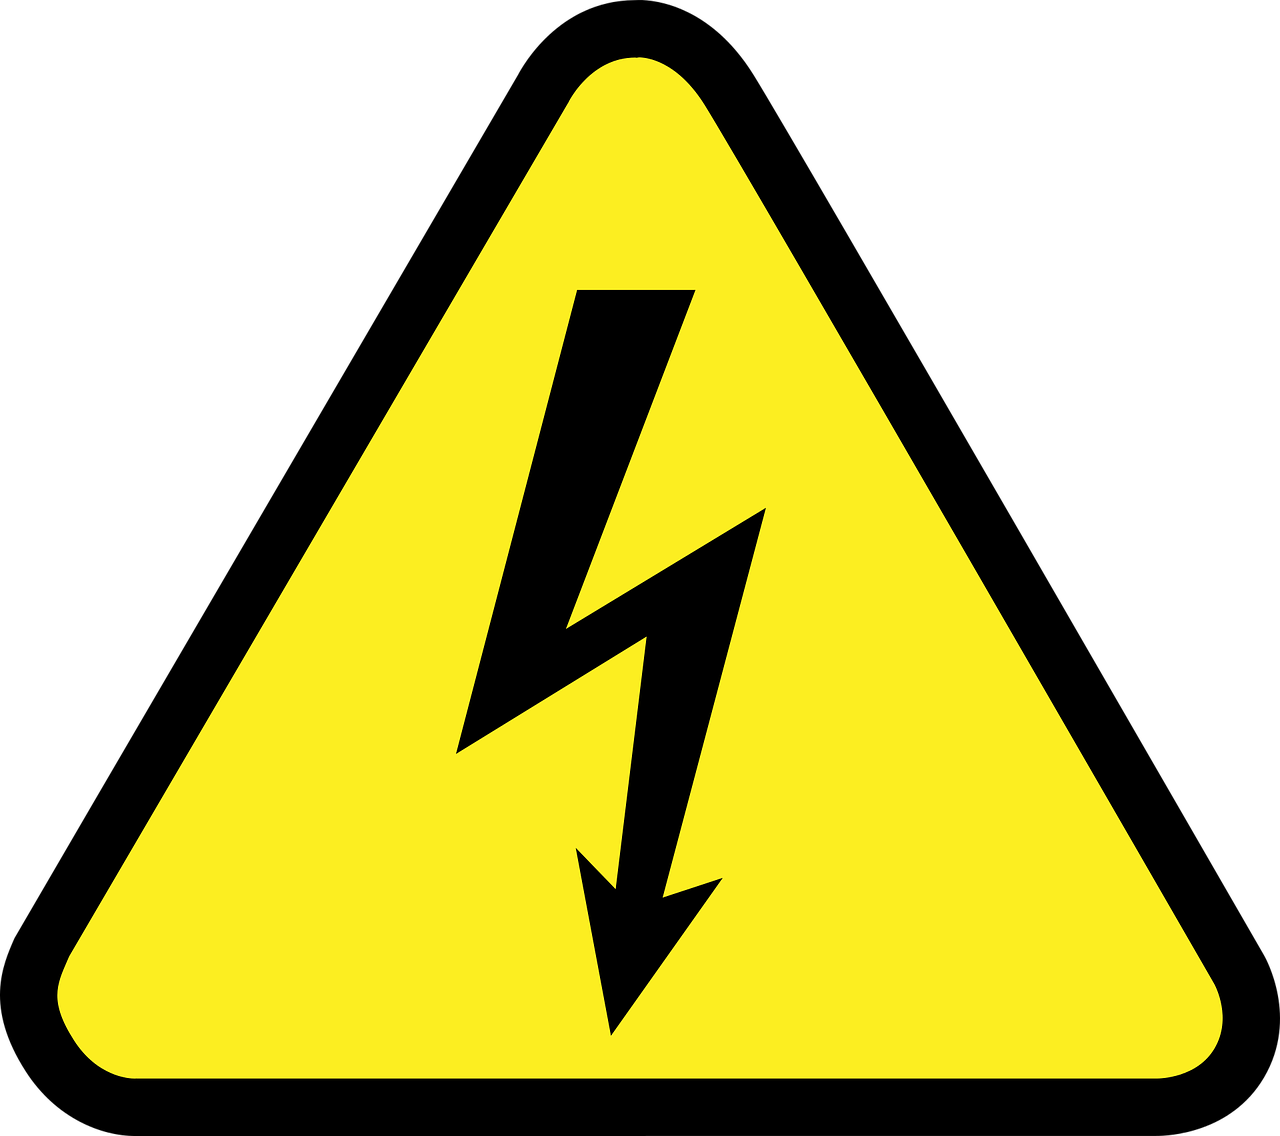
\includegraphics[width=1\textwidth]{img/hochspannung}
    \end{minipage}

\end{tcolorbox}
\end{document}
